\documentclass[tikz]{standalone}
\usepackage{pgfplots}
\pgfplotsset{compat=1.15}
\usepackage{mathrsfs}
\usetikzlibrary{arrows,calc}
\usepackage{tkz-euclide}

\pagestyle{empty}

\definecolor{AngleClr}{rgb}{0,0.39215686274509803,0}
\definecolor{ShapeClr}{rgb}{0.6,0.2,0}

\begin{document}

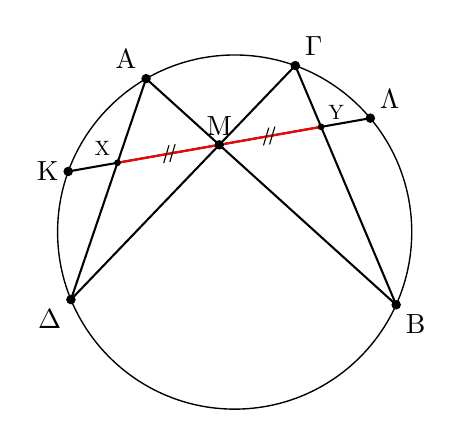
\begin{tikzpicture}[scale=.75]
\tkzSetUpLine[line width=1pt,color=black]
\tkzSetUpPoint[fill=black]

\tkzDefPoints{0/0/O}

\tkzDefPoint(40:3){L}
\tkzDefPoint(160:3){K}
\tkzDefPoint(120:3){A}
\tkzDefPoint(70:3){C}

\tkzDefMidPoint(K,L) \tkzGetPoint{M}


\tkzInterLC(A,M)(O,A) \tkzGetPoints{B}{x}
\tkzInterLC(C,M)(O,C) \tkzGetPoints{y}{D}

\tkzInterLL(A,D)(K,L) \tkzGetPoint{X}
\tkzInterLL(B,C)(K,L) \tkzGetPoint{Y}

\tkzDefPointBy[projection = onto A--B](X) \tkzGetPoint{X'}
\tkzDefPointBy[projection = onto A--B](Y) \tkzGetPoint{Y'}

\tkzDefPointBy[projection = onto C--D](X) \tkzGetPoint{X''}
\tkzDefPointBy[projection = onto C--D](Y) \tkzGetPoint{Y''}

\tkzDrawCircle[color=black,fill=white,line width=0.5pt](O,A)


\tkzDrawSegments[line width=0.75pt,color=black](A,B K,L B,C C,D A,D)
\tkzDrawSegments[line width=0.75pt,color=red](X,Y)



\tkzDrawPoints[size=3](A,B,C,D,M,K,L)
\tkzDrawPoints[size=2](X,Y)

\tkzLabelPoint[left](K){$\rm K$}
\tkzLabelPoint[above right](L){$\rm \Lambda$}
\tkzLabelPoint[above left](A){$\rm A$}
\tkzLabelPoint[below right](B){$\rm B$}
\tkzLabelPoint[above right](C){$\rm \Gamma$}
\tkzLabelPoint[below left](D){$\rm \Delta$}
\tkzLabelPoint[above](M){$\rm M$}
\tkzLabelPoint[above left,scale=0.75](X){$\rm X$}
\tkzLabelPoint[above right,scale=0.75](Y){$\rm Y$}

\tkzMarkSegments[mark=s||,size=3](X,M Y,M)


\end{tikzpicture}
\end{document}
